%%%%%%%%%%%%%%%%%%%%%%%%%%%%%%%%%%%%%%%%%
% The Legrand Orange Book
% LaTeX Template
% Version 3.1 (February 18, 2022)
%
% This template originates from:
% https://www.LaTeXTemplates.com
%
% Authors:
% Vel (vel@latextemplates.com)
% Mathias Legrand (legrand.mathias@gmail.com)
%
% License:
% CC BY-NC-SA 4.0 (https://creativecommons.org/licenses/by-nc-sa/4.0/)
%
% Compiling this template:
% This template uses biber for its bibliography and makeindex for its index.
% When you first open the template, compile it from the command line with the 
% commands below to make sure your LaTeX distribution is configured correctly:
%
% 1) pdflatex main
% 2) makeindex main.idx -s indexstyle.ist
% 3) biber main
% 4) pdflatex main x 2
%
% After this, when you wish to update the bibliography/index use the appropriate
% command above and make sure to compile with pdflatex several times 
% afterwards to propagate your changes to the document.
%
%%%%%%%%%%%%%%%%%%%%%%%%%%%%%%%%%%%%%%%%%

%----------------------------------------------------------------------------------------
%	PACKAGES AND OTHER DOCUMENT CONFIGURATIONS
%----------------------------------------------------------------------------------------

\documentclass[
	11pt, % Default font size, select one of 10pt, 11pt or 12pt
	fleqn, % Left align equations
	a4paper, % Paper size, use either 'a4paper' for A4 size or 'letterpaper' for US letter size
	%oneside, % Uncomment for oneside mode, this doesn't start new chapters and parts on odd pages (adding an empty page if required), this mode is more suitable if the book is to be read on a screen instead of printed
]{LegrandOrangeBook}

% Book information for PDF metadata, remove/comment this block if not required 


\addbibresource{sample.bib} % Bibliography file

\definecolor{ocre}{RGB}{243, 102, 25} % Define the color used for highlighting throughout the book

\chapterimage{orange2.jpg} % Chapter heading image
\chapterspaceabove{6.5cm} % Default whitespace from the top of the page to the chapter title on chapter pages
\chapterspacebelow{6.75cm} % Default amount of vertical whitespace from the top margin to the start of the text on chapter pages

%----------------------------------------------------------------------------------------
\usepackage{csquotes}
\begin{document}




%----------------------------------------------------------------------------------------
%	TITLE PAGE
%----------------------------------------------------------------------------------------

\titlepage % Output the title page
	{
\includegraphics[width=\paperwidth]{Images/background.pdf}} % Code to output the background image, which should be the same dimensions as the paper to fill the page entirely; leave empty for no background image
	{ % Title(s) and author(s)
		\centering\sffamily % Font styling
		{\Huge\bfseries TS CPRP 1 \\ Sciences de l'ingénieur\par} % Book title
		\vspace{16pt} % Vertical whitespace
		{\LARGE Séquence 2 : Représenter les pièces dans une MOCN\par} % Subtitle
		\vspace{24pt} % Vertical whitespace
		{\huge\bfseries \par} % Author name
	}









%----------------------------------------------------------------------------------------
%	SECTIONING EXAMPLES CHAPTER
%----------------------------------------------------------------------------------------


\part{Les MOCN dans le noir}

%----------------------------------------------------------------------------------------
%	MATHEMATICS EXAMPLES CHAPTER
%----------------------------------------------------------------------------------------

\chapter{Allumer le feu}

\section{Les ingrédients pour usiner}


En BTS CPRP, nous nous intéresseront au machines ayant des outils qui sont commandés numériquement par un programme informatique. Quand on achète une MOCN, elle dispose déjà d'un programme interne. Nous devons cependant le modifier pour qu'il réponde à notre besoin. Comme en informatique, chaque programme à un but précis. Nous auront en principe un programme à entrer dans la machine par pièce que nous souhaitons usiner. Pour programmer, vous connaissez sûrement déjà certain langage de programmation : on peut citer le C++, HTML, CSS, Python, Arduino, etc. Cependant les programmes utilisés pour l'usinage sont assez spécifiques et changent moins que dans d'autres domaines\footnote{Les langages de programmation pour le code ou les sites internet évoluent sans cesse, pour un codeur informatique, le choix du langage est très large par rapport à notre domaine.}. À l'origine, le langage de programmation était le \textbf{G-code}\footnote{, Développé par l'EIA (Electronic Industries Alliance) au début des années 1960.}, et finalement remplacé par l'\textbf{ISO}\footnote{Remplacé en février 1980 sous la référence RS274D.} mais certain constructeur peuvent avoir d'autre langage propre à la marque du constructeur.


\begin{figure}[H] % Use [H] to suppress floating and place the figure/table exactly where it is specified in the text
	\centering % Horizontally center the figure on the page
	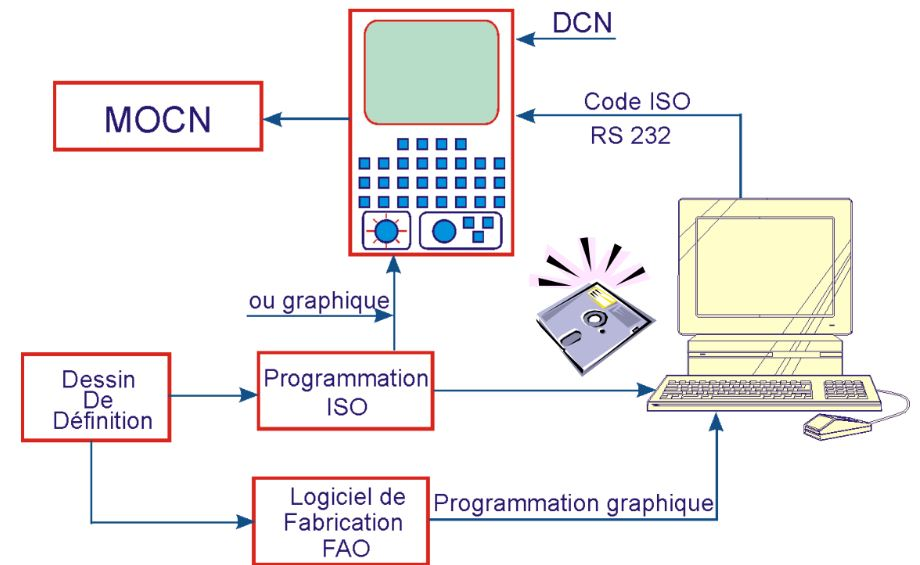
\includegraphics[width=0.7\textwidth]{Images/iso.JPG} % Include the figure image
	\caption{Chargement d'un programme dans une MOCN. Université des Sciences et de la Technologie d'Oran Mohamed-Boudiaf USTOMB}
	\label{iso3} % Unique label used for referencing the figure in-text
\end{figure}



Les machines ne sont pas comme nous, sans aucune perception de leur environnements elles sont dans le noir. Et nous leur demandons d'usiner avec une grande précision. Si on veut la longueur maximum d'une pièce de 20,001 mm mais que la pièce sortie mesure 20,002 : elle sera à jeter... Tout cela avec des vitesses très lente ou très rapide (0,001 m/min à 130 m/min). \\



Alors dans tout ça, de quoi avons-nous besoin ? \\

\begin{theorem}
\begin{itemize}
    \item Un objet de départ dont on va enlever la matière : \textit{\textbf{Le brut de matière}} ;
    \item Des éléments pour enlever la matière : \textit{\textbf{Les outils}} ;
    \item De la force ! pour trancher, percer, tronçonner, fournit par : \textit{\textbf{Des moteurs}} ; 
    \item Oui mais si j'essaye de couper une feuille de papier avec des ciseaux, sans la tenir dans l'autre main c'est difficile, il faut donc que le \textit{Brut} soit solidement "attaché" : La \textit{\textbf{MIP}} et le \textit{\textbf{MAP}}\footnote{La MIP (MIse en Position) et le MAP (MAintient en Position) seront abordés plus tard dans l'année dans différents cours, mais surtout en industrialisation.}  ;
    \item  Pour faire la forme que l'on veut : \textit{\textbf{Une trajectoire}} ;
\end{itemize}
\end{theorem}

Dans la suite nous allons nous intéresser au dernier point. \textit{Repérer les éléments dans l'espace.} 


\section{Référentiels et repères}




\section{Outil mathématique pour l'ingénieur}
Un repère du plan tout triplé où O est un point du plan et est une base. On l'écrit comme suit : $\mathcal{R}(0, \Vec{x}, \Vec{y}, \Vec{z})$. La base, c'est le tableau Excel infini, où sont présents tous les vecteur (en deux ou trois dimensions), mais ils ne peuvent pas être égaux. Par exemple, $\Vec{a}=\ \begin{Bmatrix} 1\\ 3 \end{Bmatrix} $ et $\Vec{b}=\ \begin{Bmatrix} 1\\ 3 \end{Bmatrix}$  ne peuvent pas être élus au rang de $\mathcal{B}ase$ car ils sont égaux. En revanche, dans la bibliothèque infinie il y a les vecteurs $\Vec{i}=\ \begin{Bmatrix} -1\\ 3 \\ 0 \end{Bmatrix} $ et $\Vec{j}=\ \begin{Bmatrix} -1\\ 0 \\ 3\end{Bmatrix}$ qui peuvent être choisi pour une base. \\



\begin{figure}[H] % Use [H] to suppress floating and place the figure/table exactly where it is specified in the text
	\centering % Horizontally center the figure on the page
	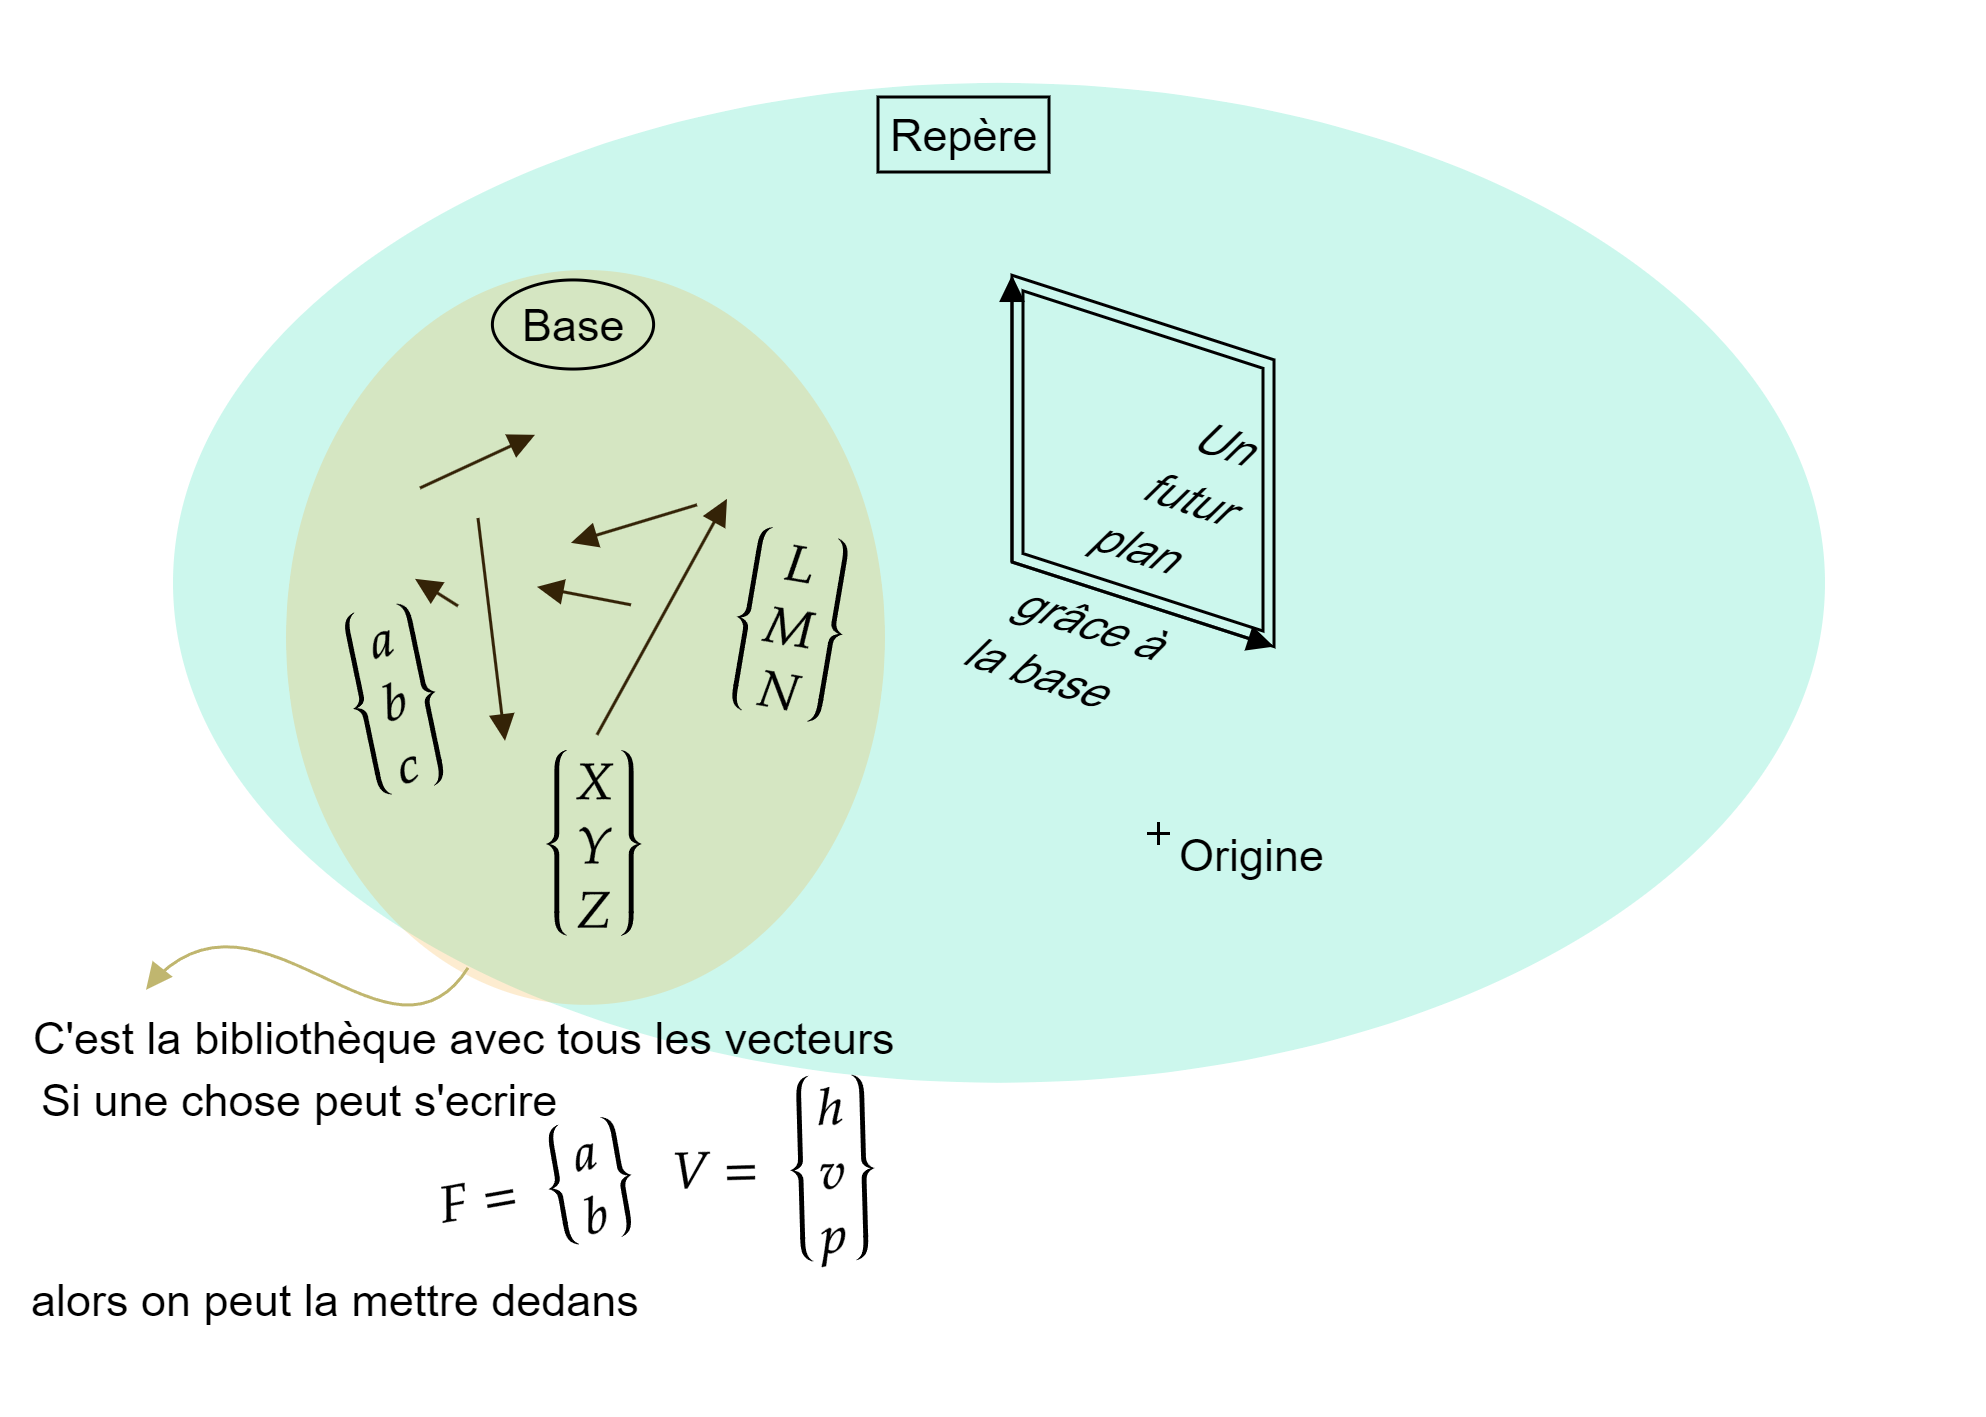
\includegraphics[width=1.1\textwidth]{Images/vect1.png} % Include the figure image
	\caption{Éléments pour construire un repère}
	\label{vect1} % Unique label used for referencing the figure in-text
\end{figure}


Un repère R est la donnée d’un point d'origine $\mathcal{O}$ et d’une base $\mathcal{B}$, permettant de repérer tous points de
l’espace par rapport à $\mathcal{O}$. On decide que $\mathcal{O}$ est notre origine, on choisi deux vecteurs dans notre bibliothèque (sauf s'il sont égaux), on prend l'origine des deux vecteurs et on le colle sur notre point $\mathcal{O}$. Voilà, le repère est fait. \\

\begin{remark}
    En pratique, nous n'avons pas besoin de dire si un vecteur ou un repère est en 2 ou 3 dimensions. Un vecteur en 2 dimensions possède 2 données $\Vec{i}=\ \begin{Bmatrix} a\\ b \end{Bmatrix} $, en trois dimension trois données : $\Vec{i}=\ \begin{Bmatrix} a\\ b \\ c \end{Bmatrix} $ \\

    Un repère en deux dimensions s'écriera $\mathcal{R}(0, \Vec{x}, \Vec{y})$, tandis-qu'un repère à trois dimensions s'écriera $\mathcal{R}(0, \Vec{x}, \Vec{y}, \Vec{z})$.
    
    Attention, si on écrire 330 c'est bien que nous nous situons dans un système de trois coordonnées.
\end{remark}

\begin{figure}[H] % Use [H] to suppress floating and place the figure/table exactly where it is specified in the text
	\centering % Horizontally center the figure on the page
	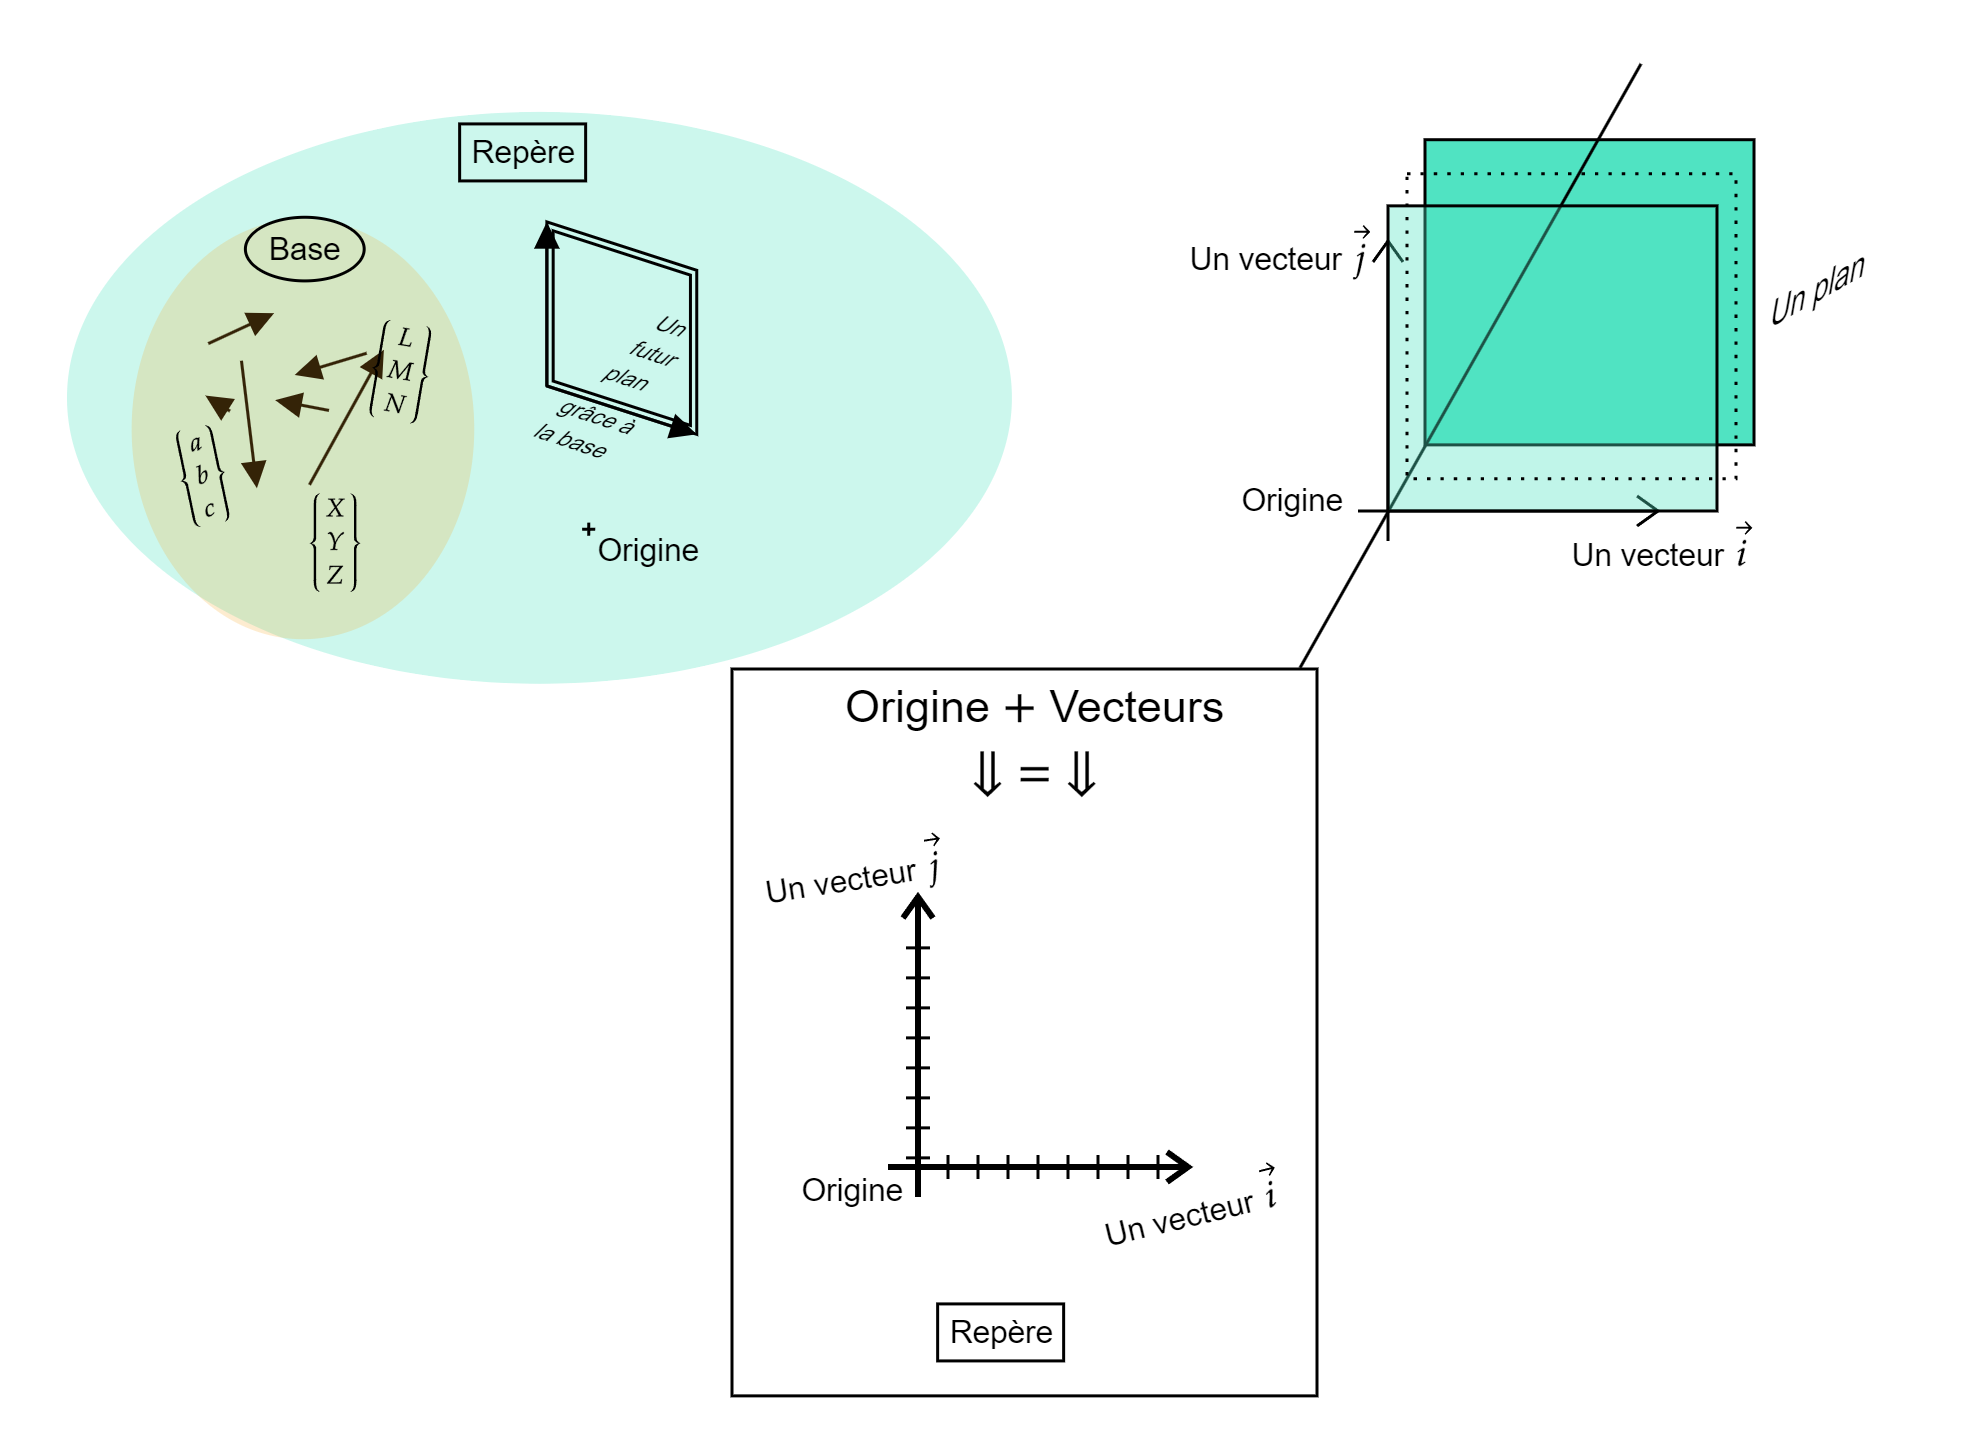
\includegraphics[width=1.1\textwidth]{Images/vect2.png} % Include the figure image
	\caption{Symbolisation d'un repère. Une fois une base (deux vecteurs) et une origine ($\mathcal{O}$) choisies, les deux vecteurs mis bout à bout forme un plan, et $\mathcal{O}$ nous sert à connaître n'importe quel point par rapprt à lui.}
	\label{vect2} % Unique label used for referencing the figure in-text
\end{figure}



Un Référentiel , on ajoute $t$, le temps avec une unité (exemple : seconde), du labo, galiéen


\section{Référentiel}

\begin{figure}[H] % Use [H] to suppress floating and place the figure/table exactly where it is specified in the text
	\centering % Horizontally center the figure on the page
	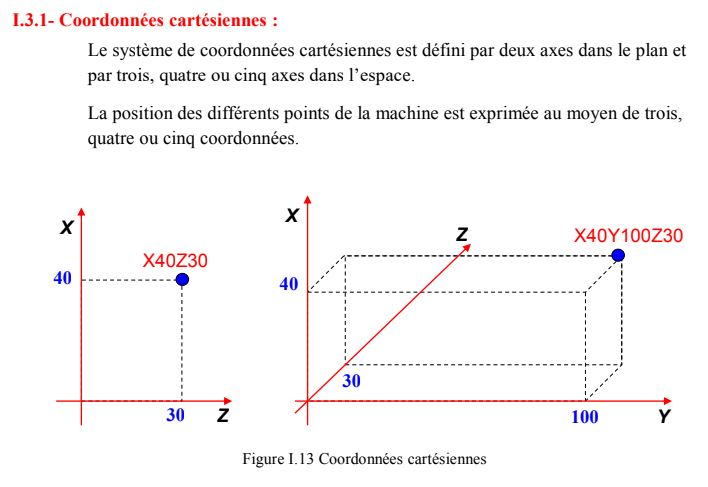
\includegraphics[width=1\textwidth]{Images/cart.JPG} % Include the figure image
	\caption{Logo de la certification QSE}
	\label{cart} % Unique label used for referencing the figure in-text
\end{figure}




\begin{figure}[H] % Use [H] to suppress floating and place the figure/table exactly where it is specified in the text
	\centering % Horizontally center the figure on the page
	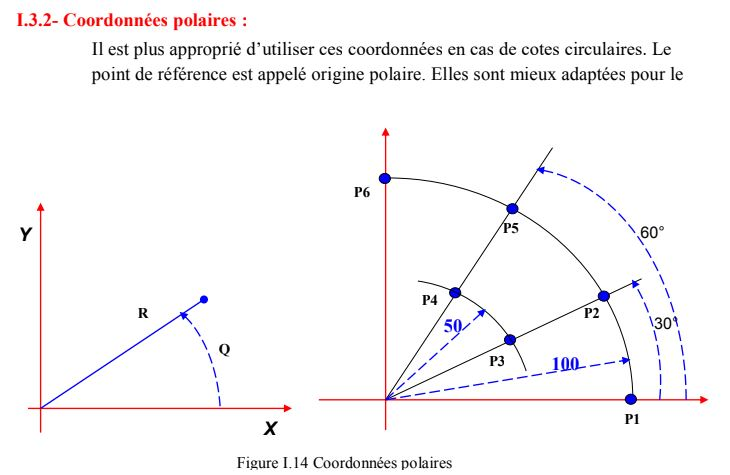
\includegraphics[width=1\textwidth]{Images/pol.JPG} % Include the figure image
	\caption{Le système de cordonnées (X, Y, Z) est un système cartésien de sens direct lié à une pièce placée sur la machine. Exemple : Sur une MOCN, on peut mettre manuellement en rotation la broche dans le sens direct en appuyant sur le bouton \textbf{C+} du pupitre de commande.}
	\label{pol4} % Unique label used for referencing the figure in-text
\end{figure}



%----------------------------------------------------------------------------------------
%	PRESENTING INFORMATION/RESULTS EXAMPLES CHAPTER
%----------------------------------------------------------------------------------------

\chapterimage{Images/chapt_F.jpg} % Chapter heading image
\chapterspaceabove{6.25cm} % Whitespace from the top of the page to the chapter title on chapter pages
\chapterspacebelow{7.5cm} % Amount of vertical whitespace from the top margin to the start of the text on chapter pages

%------------------------------------------------
\chapter{Représenter le réel}

\section{Introduction}









Pas parler de physique, rester math . un peu de math, vecteur exprime globalement tout avec une fleche ou un type de fleche (double fleche pour les moments)
\subsection{Notations}
vecteur (F ou M ou T ou V ou $\Vec{a}$ ou P), torseurs
\subsection{Vecteurs}
On écrivait comme ça,  $\Vec{i}=\ \begin{Bmatrix} a\\ b \\ c \end{Bmatrix} $  maintenant faut écrire comme ça 
 {$\mathcal{F}_{moteur} =\ \begin{Bmatrix}
F_{x}\\
F_{y}\\
F_{z}
\end{Bmatrix}_{( \mathcal{B}_{1} ,\ \vec{x} ,\ \vec{y} ,\vec{z})}$};

2D , 3D, certain sont constant $\overrightarrow{\mathcal{V}_{(train\rightarrow route)}} \ =\ C^{te}$ dautre nan $\overrightarrow{\mathcal{T}_{(train\rightarrow route)}} \ =\ X$ trajectoire



\subsection{Torseurs}
video science clic ?
\section{Position, vitesse et accélération}
Mettre le sens physique
\subsection{Vecteur trajectoire}

\section{Forces}

\section{Moments / Couples}


\begin{corollary}[S2.4] 
aze
\end{corollary}

\begin{definition}{Normes}\index{Norme}
aze
\end{definition}

\begin{theorem}
    sqdf
\end{theorem}

\begin{remark}
    aze
\end{remark}



%----------------------------------------------------------------------------------------
%	PRESENTING INFORMATION/RESULTS EXAMPLES CHAPTER
%----------------------------------------------------------------------------------------

\chapterimage{Images/A6.jpg} % Chapter heading image
\chapterspaceabove{6.25cm} % Whitespace from the top of the page to the chapter title on chapter pages
\chapterspacebelow{7.5cm} % Amount of vertical whitespace from the top margin to the start of the text on chapter pages

%------------------------------------------------


	




\newpage
\section{ANNEXE}


\phantomsection
\addcontentsline{toc}{chapter}{\textcolor{ocre}{Index}} % Add an Index heading to the table of contents
\printindex % Output the index


\end{document}


